%%%%%%%%%%%%%%%%%%%%%%%%%%%%%%
\chapter{Réalisation}
%%%%%%%%%%%%%%%%%%%%%%%%%%%%%%

%~~~~~~~~~~~~~~~~~~~~~~~~~~~~~
\section{Ergonomie de l'interface}
%~~~~~~~~~~~~~~~~~~~~~~~~~~~~~

\subsection{Mise en page}
Expliquer les div, le css ...

% Page d'options
Elle est composée d'un emboîtement de plusieurs sections, grâce à la balise HTML  \texttt{<div>}, qui est une sorte de conteneur. Comme nous l'avons précisé précédemment, nous avons séparé les options en plusieurs catégories et sous-catégories. 

\subsection{Langues}
...

%~~~~~~~~~~~~~~~~~~~~~~~~~~~~~
\section{Création d'un nouveau réseaux}
%~~~~~~~~~~~~~~~~~~~~~~~~~~~~~

\subsection{Initialisation des fichiers}
La création d'un nouveau réseaux dans WRET se fait via la page \emph{create.php}.
A partir de cette page l'utilisateur doit dans un premier temps appuyer sur le bouton \emph{Initialiser les fichiers} (Figure \ref{boutonInit}) s'il désire initialiser ses fichiers. 

\begin{figure}[!ht]
	\begin{center}
		\fbox{
   		 \begin{minipage}[c]{0.5\textwidth}
  			
\includegraphics[width=0.90\textwidth]{../Images/Rapport/creation1-1.png}  
		 \end{minipage}}
		\caption{Bouton d'initialisation des fichiers}
  		\label{boutonInit}
  	\end{center}	
\end{figure}

Ce bouton appelle le fichier \emph{initfiles.php} qui va créer les 11 fichiers nécessaires à la mise en place d'un nouveau réseau.\\
Dans ces fichiers, nous trouvons des fichiers qui seront utilisés dans le lancement de \emph{regEfmtool} (rfile, mfile, rvfile, sfile) et également des fichiers temporaires (\emph{irrevTemp}, \emph{revTemp}, \emph{reactionTemp.txt}, \emph{reactionTemp2.txt}, \emph{matrice.txt} ou encore \emph{matrice2.txt} ainsi que la base du fichier au format \emph{DAT}).\\
Tous ces fichiers sont donc créés et donnent les droits d'édition, de lecture et d'exécution à tous les utilisateurs pour ces fichiers, afin de pouvoir être modifiés sur le serveur.

\subsection{Réactions et réversibilité}
Sous la touche \emph{Initialiser les fichiers} de la page \emph{create.php}, une fenêtre de texte permet de rentrer les réactions du réseau métabolique une à une ainsi que la réversibilité de la réaction (Figure \ref{boutonAjout}). 

\begin{figure}[!ht]
	\begin{center}
		\fbox{
   		 \begin{minipage}[c]{0.7\textwidth}
  			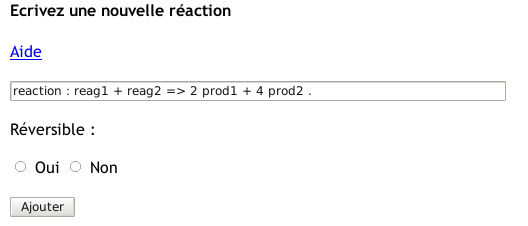
\includegraphics[width=0.90\textwidth]{../Images/Rapport/creation1-2.png}  
		 \end{minipage}}
		\caption{Bouton d'ajout d'une réaction}
  		\label{boutonAjout}
  	\end{center}	
\end{figure}

Si l'utilisateur oublie de cocher la réversibilité de la réaction et clique sur \emph{Ajouter}, un message d'erreur s'affichera et empêchera le passage à l'étape suivante. Les réactions doivent être enregistrées par l'utilisateur en respectant la syntaxe des fichier au format \emph{DAT}. Ces informations vont alors être envoyées au fichier \emph{createFiles.php}, via le bouton \emph{Ajouter}.\\
Ce fichier redirige vers différentes pages, dans l'ordre : \emph{reac.php}, \emph{parser\_enzyme.php}, \emph{parser\_reversibility.php}, \emph{parser\_metabolite.php}, \emph{parser\_stoechiometry.php}.
La première page \emph{reac.php} va permettre d'écrire dans un fichier temporaire (reactionTemp.txt) les réactions, et également, de sauvegarder la réversibilité de la réaction (0 pour non réversible, et 1 pour réversible).\\
L'ordre est ainsi conservé entre les réactions et leur réversibilité.

\subsection{Nom de réactions : enzymes}
Une fois les données de réactions et de réversibilité enregistrées, la page \emph{parser\_enzymes.php} est appelée. Elle va parser le fichier temporaire des réactions (\emph{reactionTemp.txt}) et va extraire le premier élément de la réaction situé avant le ":", qui se trouve être le nom de la réaction (nom de l'enzyme généralement).\\
Ces noms sont enregistrés dans un fichier (\emph{reaction.rfile}) en respectant les espaces et la syntaxe nécessaire à l'utilisation au sein de \emph{regEfmtool}.

\subsection{Métabolites}
Après enregistrements des enzymes, le fichier \emph{parser\_metabolites.php} est appelé. Ce script va parser le fichier temporaire contenant les réactions (\emph{reactionTemp.txt}) et va enregistrer chacun des métabolites dans un fichier (\emph{meatbolites.mfile}). Au cours de ce parsage, seuls les éléments situés après le nom de l'enzyme seront pris en compte. Les noms présents plusieurs fois dans le fichier de réactions sont enregistrés une seule fois dans le fichier \emph{metabolites.mfile}.

\subsection{Stœchiométrie}
Enfin après génération des fichiers: \emph{rvfile}, \emph{mfile}, \emph{sfile}, \emph{rfile}, le script \emph{parser\_stoechiometry} est appelé. Il va lancer le script \emph{parser\_stoechiometry.py}. Ce dernier permet de générer la matrice de stœchiométrie nécessaire a \emph{regEfmtool}. Pour ce faire, il prend les fichiers \emph{reactionTemp.txt} et \emph{metabolites.mfile} en entrée. Il génère la matrice ligne par ligne (une ligne correspondant à une réaction). \\
Pour chaque ligne du fichier \emph{reactionTemp.txt} une liste est créée et, pour chaque métabolite de cette réaction, sa stœchiométrie est enregistrée en respectant son ordre dans le fichiers contenant les réactifs. Ce script fournit alors en sortie le fichier \emph{stoechiometry.sfile}.

\subsection{Modification du réseaux}
Une fois les fichiers générés l'utilisateur est redirigé sur la page \emph{create.php}.
Sous la touche \emph{Ajouter} se trouve une zone de texte (Figure \ref{boutonAjout}) où l'utilisateur peut modifier un réseau déjà rentré. 

\begin{figure}[!ht]
	\begin{center}
		\fbox{
   		 \begin{minipage}[c]{0.7\textwidth}
  			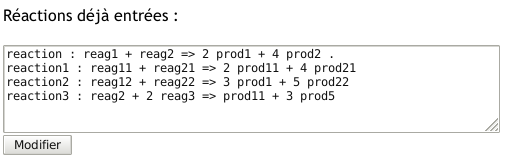
\includegraphics[width=0.90\textwidth]{../Images/Rapport/creation1-3.png}  
		 \end{minipage}}
		\caption{Bouton de modification}
  		\label{boutonModif}
  	\end{center}	
\end{figure}

En effet cette zone appelle le fichier \emph{reactionTemp.txt} et permet la modification de son contenu (pour corriger une erreur de frappe notamment). Cette zone de texte va appeler la page \emph{modifier.php} lors de l'utilisation du bouton \emph{Modifier}.\\
 Cette page efface le précédant fichier \emph{reactionTemp.txt} et insère le nouveau contenu que l'utilisateur a modifié. \\
 Les fichiers \emph{metabolites.mfile}, \emph{stoechiometry.sfile}, \emph{reactions.rfile}, \emph{reversibility}, sont également générés à nouveau, à chaque modification du fichier \emph{reactionTemp.txt}.
 
\subsection{Création du fichier \emph{DAT}}
Sous la zone de texte modifiable, un bouton \emph{DAT} permet de générer un fichier au format \emph{DAT} du réseaux métabolique précédemment rentré. \\

\begin{figure}[!ht]
	\begin{center}
		\fbox{
   		 \begin{minipage}[c]{0.3\textwidth}
  			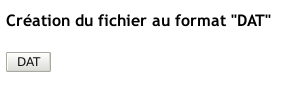
\includegraphics[width=0.90\textwidth]{../Images/Rapport/creation2-1.png}  
		 \end{minipage}}
		\caption{Bouton de création du fichier au format \emph{DAT}}
  		\label{boutonDAT}
  	\end{center}	
\end{figure}

Ce bouton (Figure \ref{boutonDAT}) appelle la page \emph{finish\_files.php} qui va concaténer trois fichiers :
\begin{itemize}
\item \emph{irrevTemp.txt}
\item \emph{revTemp.txt}
\item \emph{reactiontemp2.txt}
\end{itemize}
Le premier fichier contient l'ensemble des enzymes catalysant les réactions irréversibles. Le second contient l'ensemble des enzymes catalysant des réactions réversibles, et enfin le dernier fichier contient l'ensemble des réactions du réseaux. \\
Chacun de ces fichiers contient les balises \emph{-IRREV}, \emph{-REV}, \emph{-CAT}, selon son contenu et respecte la syntaxe propre au format \emph{DAT}.

%~~~~~~~~~~~~~~~~~~~~~~~~~~~~~
\section{Règles des gènes}
%~~~~~~~~~~~~~~~~~~~~~~~~~~~~~

La page permettant la saisie des règles générales est obtenue à l'aide du fichier \emph{generules.php}.\\
L'affichage à l'ouverture de la page n'est composé que d'une zone de texte et d'un bouton \emph{Ok} (Figure \ref{boutonOK}) qui est de type \textit{submit}. 

\begin{figure}[!ht]
	\begin{center}
		\fbox{
   		 \begin{minipage}[c]{0.3\textwidth}
  			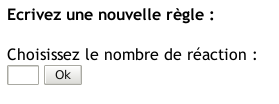
\includegraphics[width=0.90\textwidth]{../Images/Rapport/generules-1.png}  
		 \end{minipage}}
		\caption{Bouton du choix du nombre de réactions pour une règle}
  		\label{boutonOK}
  	\end{center}	
\end{figure}

Au clic, ce bouton fait appel à la fonction \emph{add\_reaction()} qui créée  deux menus déroulants (pour la première et la dernière, Figure \ref{menusDeroulants1}) ou trois menus déroulants (pour les autres, Figure \ref{menusDeroulants2}) par réaction jusqu'à atteindre le nombre de réactions entrées par l'utilisateur. 

\begin{figure}[!ht]
	\begin{center}
		\fbox{
   		 \begin{minipage}[c]{0.7\textwidth}
  			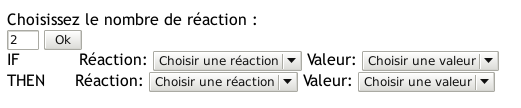
\includegraphics[width=0.90\textwidth]{../Images/Rapport/generules-2.png}  
		 \end{minipage}}
		\caption{Menus déroulant si 2 réactions dans la règle}
  		\label{menusDeroulants1}
  	\end{center}	
\end{figure}

\begin{figure}[!ht]
	\begin{center}
		\fbox{
   		 \begin{minipage}[c]{0.8\textwidth}
  			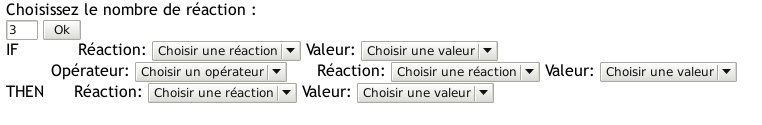
\includegraphics[width=0.90\textwidth]{../Images/Rapport/generules-3.png}  
		 \end{minipage}}
		\caption{Menus déroulant si 3 réactions dans la règle}
  		\label{menusDeroulants2}
  	\end{center}	
\end{figure}

Elle vérifie également que le nombre de réactions entrées par l'utilisateur est au moins égal à 2, sinon elle affiche un message sous la forme d'une alerte à l'utilisateur.\\
Les réactions sont récupérées à partir de \emph{reactions.rfile}.\\

L'utilisateur peut sélectionner plusieurs fois la m\^eme réaction dans sa règle, sauf pour le choix de la dernière (ligne THEN). Cette particularité est gérée par la fonction \texttt{choice(form, val)}. Celle-ci permet de remplir les menus déroulants quand une réaction a été choisie et pour la dernière seules les réactions non sélectionnées précédemment appara\^issent.

Lorsque l'utilisateur a choisi toutes ses réactions, leur opérateur et leur valeur, il clique sur le bouton \emph{Ajouter}. Celui-ci fait appel à la fonction \texttt{validateForm()} qui vérifie que tous les champs ont bien été sélectionnés. Si la fonction retourne VRAI, il fait appel au fichier \emph{createGrfile.php} qui écrit la règle dans le fichier \emph{grfile.txt}.\\
Le fichier \emph{createGrfile.php} écrit dans le fichier \emph{grfile} selon certaines règles. En effet, l'écriture de la règle dépend des valeurs associées aux réactions et des opérateurs choisis.\\

Si la valeur de la réaction qui suit le "THEN" est 0, alors il y aura le symbole "!" au début de la règle (juste après le "="), sauf si la règle ne contient que deux réactions.\\
Si les autres réactions ont pour valeur:
\begin{itemize}
\item 0, alors on écrira (!0reac)
\item 1, alors on écrira (!1reac)
\item f, alors on écrira (!freac)
\end{itemize}
En revanche, si la valeur de la réaction après "THEN" est 1, les autres réactions s'écriront:
\begin{itemize}
\item 0reac si sa valeur est 0
\item 1reac si sa valeur est 1
\item freac si sa valeur est f
\end{itemize}
De plus, si l'opérateur "AND" est sélectionné il sera écrit sous la forme \& dans le fichier, l'opérateur "OR" sera lui écrit $|$. Quand la règle est composée d'au moins trois réactions, des parenthèses sont ajoutées après chaque réaction sauf la première et la dernière. Des parenthèses entourent l'ensemble des réactions situées après le "=".\\

Pour mieux comprendre l'écriture du fichier \emph{generules.grfile}, voici un exemple:\\

Choix de l'utilisateur sur la page Web: \\
\begin{DDbox}{\linewidth}
\begin{lstlisting}
IF reaction: R1 valeur: 1
Operateur: AND reaction: R2 valeur: 0
Operateur: OR reaction: R3 valeur: 0
THEN reaction: R4 valeur: 0
\end{lstlisting}
\end{DDbox}

Règle écrite dans le fichier: \\
\begin{DDbox}{\linewidth}
\begin{lstlisting}
R4 = (!((1R1 \& (!0R2)) $|$ (!0R3))
\end{lstlisting}
\end{DDbox}


%~~~~~~~~~~~~~~~~~~~~~~~~~~~~~
\section{Choix des options de lancement}
%~~~~~~~~~~~~~~~~~~~~~~~~~~~~~

La page permettant la sélection des options de lancement est obtenue à l'aide du fichier \emph{options.php}. Comme nous l'avons dit précédemment, nous avons séparé les options en une série de catégories et sous catégories, le tout contenu dans un formulaire afin de gérer l'interaction avec l'utilisateur. Ce dernier peut sélectionner les options qu'il désire avec une combinaison de \textit{radioboutons} et de zones de texte. Les \textit{radioboutons} d'une même sous-section ont le même attribut \textit{name} afin de ne pouvoir en sélectionner qu'un seul. \\

Prenons comme exemple la première sous catégorie (Figure \ref{affichageResults}) :

\begin{figure}[!ht]
	\begin{center}
		\fbox{
   		 \begin{minipage}[c]{0.3\textwidth}
  			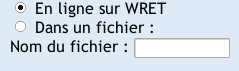
\includegraphics[width=0.90\textwidth]{../Images/Rapport/options-1.png}  
		 \end{minipage}}
		\caption{Sous catégorie d'affichage des résultats dans la catégorie d'enregistrement}
  		\label{affichageResults}
  	\end{center}	
\end{figure}

Voici le code HTML/PHP qui correspond :

\scriptsize
\begin{DDbox}{\linewidth}
\begin{lstlisting}
<input type="radio" name="choix1" value="log console" checked="checked">	<?php echo TXT_OPTIONS_SAVING_3; ?> 
<input type="radio" name="choix1" value="log file"> <?php echo TXT_OPTIONS_SAVING_4; ?> 
<?php echo TXT_OPTIONS_SAVING_5; ?> <input type="text"	 name="log_nomFichier" 	size="10" id="texte1">
\end{lstlisting}
\end{DDbox}

\normalsize

Le premier \textit{radiobouton} est pré-coché avec l'attribut \textit{checked="checked"} afin de guider l'utilisateur. Si cette option ne lui contient pas, il lui suffit de cocher le deuxième \textit{radiobouton} et de remplir la zone de texte associée. \\

Ce sont les attributs \textit{value} de ces boutons qui sont récupérés avec un script JavaScript. Ce dernier, nommé \emph{choixOptions.js}, permet de vérifier quels \textit{radioboutons} sont cochés et récupère ce qu'il a dans l'attribut \textit{value} de ceux-ci quand c'est le cas. Il est appelé lors du clic sur le bouton \textit{Lancement} en bas de la page. De plus, c'est dans ce script qu'est générée la commande qui permettra le lancement de regEfmtool. Elle est contenue dans une variable nommée  \textit{commande}, qui se remplit des paramètres sélectionnés. \\

Exemple du code JavaScript qui permet la récupération des \textit{values} précédentes : \\

\begin{DDbox}{\linewidth}
\begin{lstlisting}
var commande = "java -Xmx1G -jar ../regEfmtool.jar";

  // SAVE
  // Display
  if (formulaire.choix1[0].checked) { 
    valeur1 = " -" + formulaire.choix1[0].value; 
    commande = commande + valeur1;
  }
  else if (formulaire.choix1[1].checked) { 
    var nom1 = document.getElementById('texte1').value;
    valeur1 = " -" + formulaire.choix1[1].value + " " + nom1; 
    commande = commande + valeur1;
  }
\end{lstlisting}
\end{DDbox}

La variable \textit{commande} est une chaîne de caractères qui contient le début de la commande Java. Les paramètres sont ensuite ajoutés au fur et à mesure de la vérification de la sélection des boutons. \\

Cette commande est envoyée via un \textit{cookie} à la page d'affichage des résultats pour le lancement de regEfmtool. 

%~~~~~~~~~~~~~~~~~~~~~~~~~~~~~
\section{Chargement d'un réseau pré-existant}
%~~~~~~~~~~~~~~~~~~~~~~~~~~~~~



%~~~~~~~~~~~~~~~~~~~~~~~~~~~~~
\section{Affichage des résultats}
%~~~~~~~~~~~~~~~~~~~~~~~~~~~~~




